\documentclass[twocolumn,english]{IEEEtran}
\usepackage[T1]{fontenc}
\usepackage{babel}
\usepackage{amsthm}
\usepackage{amsmath}
\usepackage{graphicx}
\usepackage[unicode=true,
 bookmarks=true,bookmarksnumbered=true,bookmarksopen=true,bookmarksopenlevel=1,
 breaklinks=false,pdfborder={0 0 0},backref=false,colorlinks=false]
 {hyperref}
\usepackage{bm}
\usepackage{amsmath}
\usepackage{amssymb}
\usepackage{natbib}
\usepackage{array}
\usepackage{calc}
\usepackage{booktabs}
\newcolumntype{W}{>{\centering\arraybackslash}m{25mm}}
\newcolumntype{L}{>{\centering\arraybackslash}m{15mm}}


\hypersetup{
 pdftitle=  {Lab 5: Speed of Sound},
 pdfauthor= {Zack Garza},
 pdfpagelayout=OneColumn, pdfnewwindow=true, pdfstartview=XYZ, plainpages=false}

\makeatletter


%%%%%%%%%%%%%%%%%%%%%%%%%%%%%% Textclass specific LaTeX commands.
 % protect \markboth against an old bug reintroduced in babel >= 3.8g
 \let\oldforeign@language\foreign@language
 \DeclareRobustCommand{\foreign@language}[1]{%
   \lowercase{\oldforeign@language{#1}}}
\theoremstyle{plain}
\newtheorem{thm}{\protect\theoremname}
\theoremstyle{plain}
\newtheorem{lem}[thm]{\protect\lemmaname}

%%%%%%%%%%%%%%%%%%%%%%%%%%%%%% User specified LaTeX commands.
% for subfigures/subtables
\ifCLASSOPTIONcompsoc
\usepackage[caption=false,font=normalsize,labelfont=sf,textfont=sf]{subfig}
\else
\usepackage[caption=false,font=footnotesize]{subfig}
\fi

\makeatother
\providecommand{\lemmaname}{Lemma}
\providecommand{\theoremname}{Theorem}
\setcounter{topnumber}{2}
\setcounter{bottomnumber}{2}
\setcounter{totalnumber}{4}
\renewcommand{\topfraction}{0.85}
\renewcommand{\bottomfraction}{0.85}
\renewcommand{\textfraction}{0.15}
\renewcommand{\floatpagefraction}{0.7}
\usepackage{float}
\begin{document}

\title{Speed of Sound}


\author{Zack Garza}


\IEEEspecialpapernotice
{Physics 215L \\
Effective Date of Report: March 20, 2014 }


\markboth{Speed of Sound}{Zack Garza}
\maketitle
\begin{abstract}
Placeholder
\end{abstract}
\tableofcontents

\section{Introduction}
\IEEEPARstart{I}{n} this four part experiment, some interesting and important behaviors of waves will be studied and used to measure the speed of sound in three different media: air, helium, and brass.
In addition to the information covered in Chapter 14 of the text, here is an outline of this study of waves:

\begin{enumerate}
 \item Investigate the speed of waves on a string and compare the value obtained from the tension and linear density to the value derived from the frequency and wavelength.
 \item Measure the speed of sound in air and helium from time-of-flight data obtained electronically.
 \item Measure the speed of sound in air from measurements made on a standing wave in an air colum with one end open.
 An audible sound source will generate the standing wave.
 \item Measure the speed of sound in brass using a Kundt's Tube.
\end{enumerate}

\section{Theory}
%Explain each of the following.
\subsection{Characteristics and properties of transverse and longitudinal waves.}
%Draw a representation of each to add clarification.

Mechanical waves describe the phenomenon of the propagation of some disturbance through a medium. This motion causes energy to be transferred, but does not result in a net displacement of the individual particles in the medium. However, a wave may cause particles to oscillate about some equilibrium position. Depending on how these oscillations take place, waves can then be sub-categorized into two groups - transverse and longitudinal.

In a transverse wave, the individual elements of the medium move \textit{perpendicular} to the direction that wave travels -- for example, a wave traveling in the $\bf{\hat x}$ direction oscillates in any combination of the $\bf{\hat y}$ and $\bf{\hat z}$ directions. This type of motion is similar to that seen when a string is held horizontally between two points and an impulse is delivered to one end, causing a wave to travel along its length.

A longitudinal wave, however, causes the elements of the medium to move \textit{parallel} to the direction that that wave propagates. In this case, a wave traveling in the $\bf{\hat x}$ direction would cause particles in the medium to oscillate only in the $\pm\bf{\hat x}$ direction. This type of motion can be typifies a compression that travels along the length of a spring, or the propagation of a difference in pressure via sound waves.

\subsection{The relationship between the frequency and speed of a wave and its corresponding wavelength.}
%Define all symbols.

By definition, a wave travels a distance of one wavelength ($\lambda$ meters) in one period ($T$ seconds). By inspection or dimensional analysis, the speed $v$ at which the wave travels is the distance traveled divided by the time of travel, or
\begin{equation*}
 v=\lambda / T.
\end{equation*}

The frequency $f$ of a wave is defined as the number of identical points on a wave, such as crests or troughs, that pass by a given point in a unit time interval. Since waves are sinusoidal, the frequency is related to the period and
\begin{equation*}
f=1/T.
\end{equation*}

Combining the above expressions shows that the speed, frequency, and wavelength are related by the following expression:
\begin{equation}\label{eq:v.f.lambda}
 v=f\lambda
\end{equation}

When a taut string is confined between two dense materials and driven by a periodic generator, a wave traveling along the string can be reflected at the boundary and interfere with itself, which results in a \textbf{standing wave}. Each element oscillates transversely at an amplitude that depends upon its position. Points of zero amplitude are called \textbf{nodes}, while points of maximum amplitude are called \textbf{antinodes}.

Because the amplitude of standing waves are sinusoidal, the points of minimum and maximum amplitude (and thus the locations of nodes and antinodes, respectively) are periodic over $\pi$ and out of phase by $\pi/2$. This results in nodes occuring occurring at the positions $n(\lambda/2)$ for all $n \in \mathbb{N}$, and antinodes occurring at $n(\lambda/4)$ for only odd $n$. The distance between a node and an antinode is then $\lambda/4$ m, and the distance between adjacent nodes (or adjacent antinodes) is $\lambda/2$ m.

In the case of the taut string, the boundary conditions represent nodes, restricting the possible standing waves on the string to only those for which $\lambda/2 = L/n$, where $n$ is the number of loops seen in the string, representing the string's $n$th normal mode. If the length of the string is also known, the wavelength can then be found by rearranging the above expressions as
\begin{equation}\label{eq:p1_wavelength}
 \lambda = \frac{2L}{n}
\end{equation}

\subsection{The relationship for the speed of a wave on a string as a function of the string's tension and linear density.}
Consider a pulse traveling along a string at a speed $v$. A small element of the string $\Delta s$ is an arc subtended by an angle $2\theta$. The string's linear density $\mu$ is equal to its mass per unit length, which allows the mass to be expressed as $m = \mu\Delta s = \mu 2R\theta$.

From kinematics, the radial acceleration of this element equals $v^2/R$. The force of the string's tension $\bf{T}$ is exerted on the element, tangent to the arc, and the horizontal components cancel leaving a net force of $2T\sin\theta$ acting radially inward. Using the small angel approximation $\sin\theta \approx \theta$, assuming that the amplitude of the pulse is small relative to the string's length, the net radial force $F_r$ is approximately $2T\theta$.

Applying Newton's 2nd Law for circular motion and solving for $v$ yields
\begin{align}\label{eq:v.eq.t.mu}
 F_r &= ma = \frac{mv^2}{R} \Rightarrow \notag \\
 F_r &= \frac{(\mu 2R\theta)v^2}{R}  \Rightarrow \notag \\
 2T\theta &= \frac{(\mu 2R\theta)v^2}{R} \Rightarrow \notag \\
 v &= \sqrt{\frac{T}{\mu}}
\end{align}



\subsection{The Superposition Principle}

When two waves interact within a medium, they can combine either constructively or destructively, resulting in a new waveform. The superposition principle states that the resultant wave function can be expressed as the algebraic sum of the individual waves, and applies to any wave that behaves in a linear fashion. This allows to waves to occupy the same position in space and continue their motion without effecting each other. However, any particles in the medium will experience the combined effect of both waves at that spot. In mathematical terms, the superposition principle allows two displacement functions to be added together and simplified into a single function.

\subsection{The requirements for a standing wave on a string with closed boundaries.}
%Show a drawing.
\begin{figure}[h!]
  \begin{centering}
  \begin{center}
  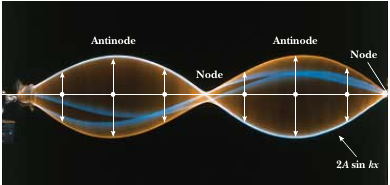
\includegraphics[width=\linewidth]{./Images/standing_wave.png}
  \label{fig:standing_wave}
  \caption{Diagram of a standing wave.}
  \end{center}
  \par\end{centering}
  \end{figure}
When the boundaries of the string are closed, the ends form nodes at which the amplitude of oscillation is necessarily zero. Because the spacing between two adjacent nodes must be an odd multiple of $\lambda/2$, any standing wave present on the string must have a wavelength that is an integral multiple of $2L$, where $L$ is the length of the string.

\subsection{The requirements for a standing wave in an air column open at one end.}
%Include a drawing
\begin{figure}[h!]
  \begin{centering}
  \begin{center}
  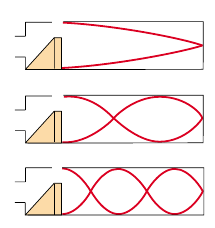
\includegraphics[width=\linewidth]{./Images/closed_open.png}
  \label{fig:closed_open}
  \caption{An air column that is closed on one end and open at the other.}
  \end{center}
  \par\end{centering}
  \end{figure}
%Are the nodes pressure or displacement nodes?
In an air column such as that depicted in Figure~\ref{fig:closed_open}, the closed boundary creates a displacement node (or a pressure antinode) and the open boundary creates a displacement anti-node (or a pressure node). Since the distance between a node and an antinode must necessarily be $\lambda/4$ for a standing wave to occur, the wavelength of the resulting wave must be $4L$ where $L$ is the length of the air column.

\subsection{The speed of sound in a gas as a function of its properties.}
%Which properties?
When a sound wave is created, it is propagated through gas mediums via longitudinal pressure waves. The speed at which such waves move depends on how compressible the gas is and now dense it is, or in a more general sense, the speed is proportional to some elastic and some inertial property of the medium. In the case of gases, the speed of a sound wave through the gas is given by
\begin{equation}
 v=\sqrt{\frac{\beta}{\rho}}
\end{equation}
where $\beta$ is the bulk modulus of the gas and $\rho$ is its density.

The speed of the wave can also be affected by the temperature of the medium. For sound in air, the speed can be calculated as
\begin{equation}
 v=(331\text{ m/s})\sqrt{1+\frac{T_C}{273^{\circ}\text{C}}}
\end{equation}
where $T_C$ is the temperature of the gas in degrees Celsius.


\subsection{The speed of sound in a solid as a function of its properties.}
%Which?
Similarly, the speed of sound in solids is also proportional to some elastic property and some inertial property. For all mechanical waves, the speed can be expressed as
\begin{equation}
 v = \sqrt{\frac{\text{elastic property}}{\text{inertial property}}}
\end{equation}

In the case of solids, the density $\rho$ is still used as the inertial property. However, the elastic property that used is Young's modulus $Y$, which represents the relationship between strain and stress on the material and in a sense also describes how ``compressible'' the material is and how it responds to mechanical disturbances. This gives the following expression for the speed of sound in a solid:
\begin{equation}
 v=\sqrt{\frac{Y}{\rho}}
\end{equation}



\section{Methodology}
\subsection*{Part 1: Waves on a String}
\begin{enumerate}
 \item The generator was started and its frequency was steadily increased until a standing wave was produced.
 %This is the fundamental, n=1
 \item Frequency was adjusted to give the maximum amplitude, and this frequency was recorded.
 \item The number of wavelengths observed in the standing wave was recorded.
 \item The frequency was increased until a second harmonic resulted, adjusted for maximum amplitude, and recorded.
 %n=2
 \item The previous step was repeated for a third harmonic.
 \item The distance $l$ from the generator to the pulley was measured.
 \item The tension mass $M_T$ was measured.
 \item The tension and length of a separate piece of string were measured.
\end{enumerate}
\subsection*{Part 2: Speed of Sound in Air and Helium}
\begin{enumerate}
 \item The oscilloscope was powered on and calibrated.
 \item A square wave generator was activated.
 \item The number of major divisions from the graticule of the scope corresponding to the time $t$ shown in the diagram were measured, along with the time base setting, and values were recorded.
 \item $L$ was measured using a two meter stick equipped with caliper jaws, where $L$ is defined on the gas tube with lines drawn at both ends.
 \item The generator was turned off, and $H_e$ gas was obtained and confined to  a beach ball fitted with surgical tubing and a hose clamp.
 \item The end of the tubing was connected to the gas inlet tube, the generator was turned on  with the same signal, the clamp was opened on the tubing and the beach ball was squeezed to force $H_e$ gas into the gas tube.
 %What happens to to the signal on the scope?
 \item Step 3 was repeated.
 \item The ambient temperature was measured.
\end{enumerate}

\subsection*{Part 3: Speed of Sound from a Standing Wave}
\begin{enumerate}
 \item The level control was unclamped and raised until the water level was close to the top of the column, and then reclamped.
 \item The amplitude knob on the generator was adjusted to its lowest setting.
 \item The generator was turned on and set to a frequency of 426 Hz.
 \item The frequency was turned up until the sound produced was audible with a low intensity.
 \item The generator was fine tuned by striking a 426.6 Hz tuning fork, listening for beats, and adjusting the generator frequency until the beats disappeared.
 \item The water level was lowered to produce an increase in sound intensity, and adjusted until the intensity was at a maximum. The water level was then recorded for $L_1$.
 \item The last step was repeated for $L_2$.
 \item The room temperature was measured and recorded.
\end{enumerate}

\subsection*{Part 4: Speed of Sound in Brass}
\begin{enumerate}
 \item The dust in the Kundt's tube was redistributed evenly along the tube, without touching the brass rod.
 \item The brass rod was clamped at its midpoint. %TODO: Why?
 \item The rosin cloth was wrapped around the brass rod to the left of the clamp, with the rosin side contacting the brass.
 \item The cloth was gripped and pulled along the brass rod to produce a high pitched sound.
 \item This was continued until the cork dust settled into a pattern that did not change between pulls.
 \item A reference point was selected at one end of the tube, and a corresponding point matching the dust pattern was selected on the other end of the tube.
 \item The two points were marked with a felt tip marker and the distance between them was recorded with a meter stick.
 \item The number of wavelengths over this distance was counted and recorded.
 \item The distance between the left end of the brass rod and the point of contact between the clamp and the rod was measured.
 \item The room temperature was measured and recorded.
\end{enumerate}


\section{Data}
  \subsection*{\textbf{Part 1}}
  \begin{table}[h]
  \centering{}
  \begin{tabular}{|l|l|l|}
  \hline
  n & Frequency (Hz)		& \# Wavelengths 	\\ \hline
  1 & $57.4$	            	& $1$                	\\ \hline
  2 & $113.8$               	& $2$               	\\ \hline
  3 & $171.1$               	& $3$              	\\ \hline
  \end{tabular}
  \end{table}

  \begin{align*}
   l   &= \text{\underline{$307.0$ cm}}	&	L&= \text{\underline{$89.3$ cm}} \\
   M_s &= \text{\underline{$1.07$ g}} 	&	M_T&= \text{\underline{$553.31$ g}}
  \end{align*}

  \subsection*{\textbf{Part 2}}
  \begin{align*}
   &\text{\textbf{Air:}}	&\text{\# of divisions: } &\text{\underline{$5.10$ divs} }	& &\text{\# s/div: \underline{$1$ ms/div}} \\
   &\text{\textbf{He:}}		&\text{\# of divisions: } &\text{\underline{$2.50$ divs} }		& &\text{\# s/div: \underline{$1$ ms/div}}
  \end{align*}
  \begin{align*}
   &L = \text{\underline{$140.2$ cm}}	&T = \text{\underline{$24.0^{\circ}$ C}}
  \end{align*}


  \subsection*{\textbf{Part 3}}
  \begin{align*}
   &\text{Frequency: \underline{$426.6$ Hz?}} 			&\text{$L_1 =\,$\underline{$72.7$}} \\
   &\text{Temperature: \underline{$24.0\,^{\circ}$C}}		&\text{$L_2 =\,$\underline{$32.5$}}
  \end{align*}

  \subsection*{\textbf{Part 4}}
  \begin{align*}
   &\text{Distance Between Patterns:} 	&\text{\underline{$8.51$ cm}} \\
   &\text{Length of Cork Dust Pattern:} &\text{\underline{$62.3$ cm}} \\
   &\text{Number of Wavelengths:} 	&\text{\underline{$8$}} \\
   &\text{Length of Brass Rod:} 	&\text{\underline{$(44.5\pm0.5)$ cm}} \\
   &\text{Room Temperature:} 		&\text{\underline{$24.0\,^{\circ}$ C}}
  \end{align*}

\section{Analysis}
\subsection*{Part 1}

\begin{table}[h]
\centering
\caption{Wave Speed Calculations (From Equations~\ref{eq:p1_wavelength} and~\ref{eq:v.f.lambda})}
\begin{tabular}{@{}lll@{}}
\toprule
\textbf{Normal Mode} & \multicolumn{1}{c}{\begin{tabular}[c]{@{}c@{}}$\lambda$\\ (m)\end{tabular}} & \multicolumn{1}{c}{\begin{tabular}[c]{@{}c@{}}$v$\\ (m/s)\end{tabular}} \\ \midrule
1                    & 1.98                                                                        & 113.71                                                                  \\
2                    & .9905                                                                       & 112.72                                                                  \\
3                    & .6603                                                                       & 112.98
\\ \bottomrule
\textbf{Average}     & \multicolumn{1}{c}{N/A}                                                     & \multicolumn{1}{c}{113}                                                 \\ \bottomrule
\end{tabular}
\end{table}

\textbf{Linear Density: }

$\mu = \frac{M_{\text{String}}}{L} = \frac{.00107\text{ kg}}{3.070\text{ m}} = $
\underline{ .000349{ kg/m}}

\textbf{String Tension: }

$T = (.55331\text{ kg})(9.80\text{ m/s}) =$ \underline{5.42 N}

\textbf{Wave Speed: }

$v = \sqrt{\frac{T}{\mu}} = \sqrt{\frac{5.42\text{ N}}{.000349 \text{ kg/m}}} =$
\underline{124.70 m/s} \\%TODO

\noindent\hrulefill
\begin{align*}
 &\text{Speed of String Wave (Standing Wave): } &\text{\underline{$113$ m/s}} \\
 &\text{Speed of String Wave (Properties): }	&\text{\underline{$125$ m/s}} \\
 &\text{Percent Error: } 			&\text{\underline{$9.6$\%}}
\end{align*}
\noindent\hrulefill

\subsection*{Part 2}

\textbf{Time of Flight (Air)}

($5.10$ divs)($1$ ms / div) = 5.10 ms

\textbf{Speed of Sound in Air}

$v_{\text{Measured}}=\frac{2L}{t}=\frac{2(.9960\text{ m})}{5.10\text{ ms}} = 390.5$ m/s

$v_{\text{Theory}} = 331.5 + .607(24.0^{\circ}\text{ C}) = 346.1$ m/s

\textbf{Time of Flight (Helium)}

($2.50$ divs)($1$ ms / div) = 2.50 ms

\textbf{Speed of Sound in Helium}

$v_{\text{Measured}}=\frac{2L}{t}=\frac{2(.9960\text{ m})}{2.50\text{ ms}} = 796.8$ m/s


\noindent\hrulefill
\begin{align*}
 &					&\text{\textbf{Air}}	&	&\text{\textbf{He}}	\\
 &\text{Speed of Sound (Calculated)} 	&\text{\underline{$391$}} &	&\text{\underline{$797$ m/s}} \\
 &\text{Speed of Sound (Theoretical)\cite{serway2013physics}} 	&\text{\underline{$346.1$}} &	&\text{\underline{$972$ m/s}} \\
 &\text{Percent Error}			&\text{\underline{$13\%$}}	&	&\text{\underline{$-18\%$}}
\end{align*}
\noindent\hrulefill

\subsection*{Part 3} %Done
\textbf{Distance Between Antinodes: }

$\Delta L = 40.2$ cm

\textbf{Wavelength: }

$\lambda/2 = \Delta L \Rightarrow \lambda = 2(.402\text{ m}) = .804$ m

\textbf{Speed of Sound in Air (Calculated): }

$v_{\text{Calc}} = f\lambda = (426.6\text{ Hz})(.804\text{ m}) = 343$ m/s

\textbf{Speed of Sound in Air (Given): }

From Part 2: 346.1 m/s

\noindent\hrulefill
\begin{align*}
 &\text{Speed of Sound in Air (Calculated):}	&\text{\underline{$343$ m/s}} \\
 &\text{Speed of Sound in Air (Accepted):}	&\text{\underline{$346.1$ m/s}} \\
 &\text{Percent Error:}				&\text{\underline{$-0.9 \%$}}
\end{align*}
\noindent\hrulefill

\subsection*{Part 4}
\textbf{Wavelength of Sound in Tube}

$\lambda_{\text{Air}} = \frac{\text{Pattern Length}}{\text{\# Wavelengths}} = \frac{.623\text{ m}}{8\text{ Wavelengths}} = .07787$ m

\textbf{Speed of Sound in Air}

$v_{\text{Sound in Air}} = 331.5 + .607(24.0^{\circ}\text{ C}) = 346.1$ m/s

\textbf{Sound Frequency}

$f =\frac{v}{\lambda_{\text{Air}}}\Rightarrow f=\frac{346.1\text{ m/s}}{.07787\text{ m}} =4445$ Hz

\textbf{Wavelength of Sound in Brass}

$\frac{1}{2}(\lambda_{\text{Brass}})=(\text{Length Brass to Clamp}) \Rightarrow$

$\lambda_{\text{Brass}} = (2)(.445\text{ m}) = .890$ m

\textbf{Speed of Sound in Brass}

$v_{\text{Sound in Brass}} = f\lambda_{\text{Brass}} = (4445\text{ Hz})(.890\text{ m}) = 3956$ m/s


\noindent\hrulefill
\begin{align*}
 &\text{Speed of Sound in Brass:}				&\text{\underline{$3960$ m/s}} \\
 &\text{Speed of Sound, Accepted\cite{serway2013physics}: }	&\text{\underline{$4700$ m/s}} \\ %Cite Source
 &\text{Percent Error}						&\text{\underline{$16\%$}}
\end{align*}
\noindent\hrulefill

\section{Conclusion}
\textbf{Questions}
\begin{enumerate}
 \item \textit{Why does the brass respond to the rosin cloth by producing sound?}

  When the rosin is pulled along the rod, a process of stick-slip friction induces oscillations that cause the rod to resonate at its fundamental frequency. At any given moment, molecules in the lattice of the rod are being pulled from their equilibrium positions, supplying them with potential energy. When the cloth continues its motion, the molecules are released. The potential energy is converted to kinetic energy, and they oscillate about their equilibrium position in a damped manner. This produces a specific tone, much like pulling a bow across violin or plucking a string.\\

 \item \textit{What is the significance of the clamp?}
  The clamp causes a standing wave to be set up within the rod, forcing the center of the rod to be a node and the ends to be antinodes. Because the distance between nodes and antinodes must always be $\lambda/4$, this allows the total wavelength of the sound produced by the rod to be related to the length, giving the equation $\lambda = 2L$. \\

 \item \textit{Why does the brass rod have to be clamped at its midpoint?}

  This creates a node directly in the center of the rod, which in turn centers the longitudinal wave about the rod's center and forces the wavelength of the standing wave to be twice the length of the rod.\\
  .
 \item \textit{Why does the cork dust pile up?}

 The piles of dust denote the spots within the tube that are nodes of the standing sound wave that is created. The pressure varies everywhere else within the tube, disturbing the dust. After several seconds of this, the dust settles into these nodes, where there is no disturbance in the air immediately surrounding them. \\

 \item \textit{How do the measurements made lead to the speed of sound in brass?}

 The boundary conditions of the rod consist of a node at the center and an antinode at each end, which allows the wavelength to be determined in terms of the rod's physical length. The waves that enter the tube are at the same frequency as those that leave the rod due to the fact that the frequency produced is a characteristic of the source. A standing wave is then set up in the tube, and the distance between the nodes is measurable. Both waves obey the equation $v=f\lambda$, and since the speed of sound in air is known, as are the wavelengths of the standing waves in the tube and in the rod, the speed of sound in brass can be expressed in two equations and two unknowns and solved for. \\
\end{enumerate}

\appendices{}

\bibliographystyle{plain}
\bibliography{physbib}

\end{document}